% LEON: LLM-Enabled Intent-Driven Operations for LEO Mega-Constellations
% Target: IEEE INFOCOM 2027
\documentclass[10pt, conference, letterpaper]{IEEEtran}

\usepackage{amsmath,amssymb,amsfonts}
\usepackage{algorithmic}
\usepackage{graphicx}
\usepackage{textcomp}
\usepackage{booktabs}
\usepackage{multirow}
\usepackage{cite}
\usepackage{url}
\usepackage{xcolor}
\usepackage{enumitem}
\usepackage{adjustbox}
\usepackage{tikz}
\usetikzlibrary{positioning, arrows.meta, calc}

% Semantic macro for validator decisions (avoids \textsc font issues)
\newcommand{\decision}[1]{\textsf{\MakeUppercase{#1}}}

\usepackage{amsthm}
\newtheorem{definition}{Definition}
\newtheorem{theorem}{Theorem}

\begin{document}

\title{LEON: LLM-Enabled Intent-Driven Operations\\for LEO Mega-Constellations}

\author{\IEEEauthorblockN{Yuanhang Li}}

\maketitle

% ============================================================
\begin{abstract}
Large LEO mega-constellations already carry diverse services---remote
sensing data relay, telemetry tracking and command (TT\&C), and
latency-sensitive financial traffic---yet translating operator
requirements into routing constraints remains largely manual.
Three problems grow acute as constellation scale increases.
First, operator intents that combine multiple conditions
(latency bounds, region avoidance, node maintenance) are difficult
to parse correctly with rule-based methods, which degrade sharply
on compositional requests.
Second, an incorrectly compiled constraint can silently disable
critical links or violate safety margins, risking service outages
for mission-critical traffic.
Third, when disruptions such as solar storms or equipment failures
demand rapid reconfiguration, route computation on the constrained
topology must be fast enough for real-time response.

We present \textbf{LEON} (LLM-Enabled Intent-Driven Operations for
LEO Networks), an intent-driven routing framework that addresses
these challenges with three matched components.
An LLM-based intent compiler built on Qwen3.5-9B converts
natural-language operator requests into a typed constraint
intermediate representation, achieving 86.2\% full semantic match
on a 240-intent benchmark and outperforming rule-based parsing
by 59.0 percentage points on compositional intents.
A deterministic 8-pass validator checks structural correctness,
semantic consistency, and physical feasibility before any constraint
reaches the routing layer, accepting no unsafe intents across all
evaluation scenarios.
A lightweight GNN cost-to-go router executes validated constraints
on a Walker Delta 20$\times$20 constellation, delivering 99.8\%
packet delivery ratio with 17$\times$ inference speedup over
Dijkstra.
End-to-end experiments across four constrained scenarios---node
failure, plane maintenance, polar avoidance, and compositional
constraints---confirm zero constraint violations.
\end{abstract}

\begin{IEEEkeywords}
LEO satellite networks, intent-based networking, graph neural networks,
large language models, constrained routing, formal verification
\end{IEEEkeywords}

% ============================================================
\section{Introduction}
\label{sec:intro}

Large low Earth orbit (LEO) constellations are becoming critical
infrastructure for global connectivity, remote sensing backhaul,
and resilient space information services~\cite{leo_constellation_survey}.
As these systems scale, network operation extends well beyond
computing routes over a known topology. Operators must frequently
translate mission-level requirements into concrete routing actions
under time pressure. A remote sensing task may require bulk image
data to be relayed around congested regions before a downlink window
closes; telemetry, tracking, and command (TT\&C) traffic may need
protected low-latency paths during critical maneuvers; and emergency
conditions such as solar storms or equipment failures may demand
immediate rerouting away from affected inter-satellite links (ISLs).
Conventional configuration workflows---manually written policies and
static routing rules---can handle these cases individually, but they
become increasingly difficult to adapt quickly and consistently as
constellation size, service diversity, and failure modes
grow~\cite{satnet_ops}.

This growing operational complexity motivates higher-level control
abstractions. Intent-based networking (IBN) has been widely studied
in terrestrial networks as a way to let operators specify \emph{what}
they want while the system determines \emph{how} to enforce
it~\cite{ibn_survey,ibn_framework}. In parallel, satellite networking
research has investigated software-defined control and dynamic routing
for non-terrestrial networks~\cite{satellite_sdn_survey,leo_routing_survey}.
These two lines of work are complementary but do not directly solve
the operational problem above: terrestrial IBN methods assume
comparatively stable topologies and do not model orbital
dynamics~\cite{ibn_template,ibn_ontology}, while satellite control
frameworks typically require structured policy inputs rather than
free-form requests that must be compiled, checked, and executed
safely end to end.

This paper studies that missing step: converting operator intent into
safe and efficient routing actions for large LEO constellations. We
focus on a Walker Delta $20\times20$ constellation (400~satellites,
550\,km altitude, 53\textdegree\ inclination) and identify three
coupled challenges:

\begin{enumerate}[leftmargin=*]
\item \textbf{Semantic translation.} Operational requests naturally
combine multiple constraints in one statement---traffic class,
excluded regions, latency budgets, failover conditions---especially
when an operator must simultaneously prioritize TT\&C while avoiding
storm-exposed polar links, or redirect remote sensing relay traffic
while preserving path diversity. Rule-based parsers handle simple
single-constraint intents but degrade sharply on such compositional
requests (40.0\% vs.\ 99.0\% accuracy in our evaluation).

\item \textbf{Safety and feasibility.} In satellite networks, an
incorrect or infeasible policy is not merely an optimization error.
A mistranslated intent can route TT\&C traffic onto unstable paths,
delay time-sensitive sensing data, or prohibit links that are
topologically necessary after failures. Accepting an infeasible
policy can create routing blackholes or disconnect critical traffic
classes. Safety therefore requires that invalid or operationally
dangerous intents be kept off the certified execution path---either
explicitly rejected or deferred to conservative fallback routing.

\item \textbf{Execution efficiency.} Even after compilation and
verification, the network must produce routing decisions quickly
enough for real-time response. Exact shortest-path procedures deliver
high-quality routes but become a bottleneck when operators need rapid
reconfiguration across a 400-node time-varying constellation during
solar-storm exposure or satellite failures.
\end{enumerate}

To address these challenges, we present \textbf{LEON}
(\textbf{L}LM-\textbf{E}nabled Intent-driven \textbf{O}perations
for LEO \textbf{N}etworks), an end-to-end framework for safe
intent-driven routing in large satellite constellations
(Fig.~\ref{fig:system_architecture}). LEON makes
the challenge-to-solution mapping explicit:
\begin{itemize}[leftmargin=*]
\item For \emph{semantic translation}, LEON uses an LLM-based intent
compiler (Qwen3.5-9B) that converts natural-language operator
requests into a typed constraint intermediate representation,
achieving 86.2\% full semantic match and outperforming rule-based
parsing by 59.0 percentage points on compositional intents.
\item For \emph{safety and feasibility}, LEON introduces a
deterministic 8-pass validator that checks structural correctness,
semantic consistency, and constructive feasibility before any
constraint reaches the routing layer, accepting no unsafe intents
in our evaluation.
\item For \emph{execution efficiency}, LEON employs a lightweight
GNN cost-to-go router (152K parameters) that approximates
Dijkstra-quality routing with 17$\times$ inference speedup,
delivering 99.8\% packet delivery ratio.
\end{itemize}

\noindent End-to-end evaluation across four constrained
scenarios---node failure, plane maintenance, polar avoidance, and
compositional constraints---confirms zero constraint violations with
both GNN and heuristic Dijkstra fallback routing. The LLM
compiler further retains 81.8\% accuracy on 33 scorable
out-of-distribution paraphrases (4.4pp degradation), demonstrating
robustness to phrasing variation.

Our contributions are:
\begin{itemize}[leftmargin=*]
\item We formulate safe intent-driven operation for large LEO
satellite networks and present LEON, an end-to-end architecture
connecting natural-language intent compilation, deterministic safety
validation, and fast constrained routing. Unlike terrestrial IBN
systems~\cite{ibn_survey,ibn_framework} and prior satellite control
frameworks~\cite{satellite_sdn_survey,leo_routing_survey}, LEON is
designed specifically for dynamic constellation topology and
mission-critical traffic.
\item We design an LLM-based intent compiler that captures
compositional operator requests with 86.2\% full semantic match,
59.0pp improvement over rule-based parsing on compositional cases,
and 81.8\% accuracy on out-of-distribution paraphrases.
\item We develop a deterministic 8-pass validator that blocks
structurally invalid, semantically inconsistent, or infeasible
intents from certified acceptance (via explicit rejection or
abstention to conservative fallback routing), achieving 0\% unsafe acceptance and
grounding safety in operationally meaningful satellite-network
constraints.
\item We introduce a compact GNN cost-to-go router for efficient
constrained routing, achieving 99.8\% packet delivery ratio and
17$\times$ speedup, while the full LEON pipeline maintains zero
constraint violations across four operational scenarios.
\end{itemize}

The rest of this paper is organized as follows.
Section~\ref{sec:related} reviews related work.
Section~\ref{sec:system} presents the system model and overall LEON
architecture. Section~\ref{sec:eval} reports experimental
results. Section~\ref{sec:discussion} discusses design trade-offs
and limitations, and Section~\ref{sec:conclusion} concludes the paper.

% ============================================================
\section{Related Work}
\label{sec:related}

To position LEON with respect to prior literature, we review the
lines of work most relevant to this paper. Our goal is not only to
summarize existing methods, but also to clarify what they do well,
where they fall short, and why an end-to-end framework for
intent-driven LEO operation is still needed. We organize the
discussion into five categories: LEO constellation routing, GNN-based
network optimization, intent-based networking, LLMs for network
management, and intent-driven satellite networking.

\noindent\textbf{LEO constellation routing.}
Routing in LEO constellations has been studied through snapshot-based
shortest-path methods~\cite{snapshot_routing}, contact-graph routing
(CGR)~\cite{cgr}, and learning-based
approaches~\cite{drl_leo1,drl_leo2}. These methods capture the
distinctive structure of satellite networks---predictable mobility,
intermittent visibility, and constrained path diversity---and are
effective when the routing objective is already specified in
algorithmic form. Their limitation is that they generally assume
structured inputs designed by experts: they solve \emph{how} to
compute routes once constraints are known, but not \emph{how} to
translate operator requests such as TT\&C protection or emergency
avoidance into those constraints safely and consistently.

\noindent\textbf{GNN-based network optimization.}
Graph neural networks have shown strong performance in traffic
engineering~\cite{gnn_te}, link scheduling~\cite{gnn_scheduling},
and routing approximation~\cite{gnn_routing,routenet} by exploiting
graph structure while remaining efficient at inference time. Their
main advantage is scalability: once trained, a GNN can approximate
expensive optimization procedures much faster than iterative solvers.
However, most GNN-based network optimizers target terrestrial settings
(WANs, data centers) where topology and control objectives differ
substantially from LEO constellations. Moreover, these works begin
from pre-specified constraints and do not address whether those
constraints were derived correctly from high-level intent, nor do
they provide safety screening before deployment.

\noindent\textbf{Intent-based networking.}
Intent-based networking (IBN), also discussed as intent-driven
networking (IDN), aims to let operators specify desired outcomes
instead of low-level
configurations~\cite{ibn_survey,ibn_framework}. Prior work has
explored templates~\cite{ibn_template},
ontologies~\cite{ibn_ontology}, domain-specific
languages~\cite{nile}, and LLM-based
translation~\cite{llm_network1,llm_network2}. The benefit is
abstraction: it reduces operator burden and improves consistency.
The limitation is that many systems rely on fixed schemas or
controlled vocabularies, reducing flexibility for compositional or
varied natural-language intents. Most terrestrial IBN systems also
assume stable infrastructure and do not model the feasibility
constraints introduced by orbital dynamics, sparse inter-plane
connectivity, or mission-dependent traffic criticality.

\noindent\textbf{LLMs for network management.}
LLMs have been explored for configuration
generation~\cite{llm_config}, anomaly
diagnosis~\cite{llm_anomaly}, and policy
translation~\cite{llm_policy,netllm,llm_netops}. Their key
advantage over template-based IBN is flexibility: they can interpret
varied and compositional language with less manual schema design.
The corresponding drawback is reliability---LLM outputs may be
incomplete, inconsistent, or hallucinated, and most current systems
lack end-to-end safety guarantees. This is particularly problematic
in satellite operations, where a mistranslated intent may misroute
TT\&C traffic or accept a topologically impossible policy.

\noindent\textbf{Intent-driven satellite networking.}
Several recent studies apply IBN/IDN concepts to satellite or
non-terrestrial networks, including software-defined satellite
networking, service orchestration, and integrated
space-air-ground systems~\cite{satellite_ibn,satellite_idn,ntn_orchestration}.
These efforts recognize that future satellite systems need
higher-level control abstractions. Their strength lies in bringing
intent concepts into a domain with dynamic topology and heterogeneous
services. However, most focus on architectural frameworks or
structured service requests rather than free-form intent compilation
for constrained routing, and many leave verification at a conceptual
level.

\textbf{Summary.} The literature is rich but fragmented. LEO routing
research provides strong execution mechanisms but assumes
expert-crafted constraints. Terrestrial IBN and LLM-based management
improve the operator interface but do not address the safety and
feasibility issues of dynamic LEO topologies. Emerging intent-driven
satellite networking brings the right application perspective but
stops short of a complete compiler--validator--router pipeline. LEON
fills this gap by integrating these three capabilities in a single
framework, enabling natural-language intents for remote sensing relay,
TT\&C protection, and emergency rerouting to be translated, checked,
and enforced with explicit safety control.

% ============================================================
\section{System Design}
\label{sec:system}

Building on the gaps identified above, this section presents the
LEON framework. We first formulate the problem and introduce the
notation used throughout the paper (Table~\ref{tab:notation}), then
describe each component in the order it appears in the pipeline:
intent compilation, deterministic validation, and constrained routing.

\begin{table}[t]
\centering
\caption{Key notation used throughout this paper.}
\label{tab:notation}
\small
\begin{tabular}{cl}
\toprule
\textbf{Symbol} & \textbf{Description} \\
\midrule
$P, S, N$ & Orbital planes, satellites per plane, total nodes \\
$K$ & Max ISL neighbors per satellite (=4) \\
$G_t = (V, E_t)$ & Constellation graph at time $t$ \\
$\ell$ & Natural-language operator intent \\
$\mathcal{P}$ & ConstraintProgram (typed IR) \\
$\mathcal{F}, \mathcal{H}, \mathcal{S}$ & Flow selectors, hard/soft constraints \\
$M_V, M_E$ & Node mask, edge mask after grounding \\
$\mathbf{u}, \mathbf{d}$ & Utilization caps, flow deadline values \\
$\Gamma$ & Grounding function \\
$\Pi$ & Next-hop routing table \\
$\iota$ & Orbital inclination angle \\
$\mathcal{P}^{\checkmark}$ & Validated ConstraintProgram \\
$\odot$ & Element-wise masking operator \\
$\mathcal{R}, \mathcal{T}$ & Region name set, traffic class set \\
$G'_t$ & Constrained subgraph after mask application \\
\bottomrule
\end{tabular}
\end{table}

% System architecture figure (spans both columns)
% System Architecture Figure (TikZ)
% Single-row layout with adjustbox for precise width control

\begin{figure*}[t]
\centering
\begin{adjustbox}{max width=\textwidth}
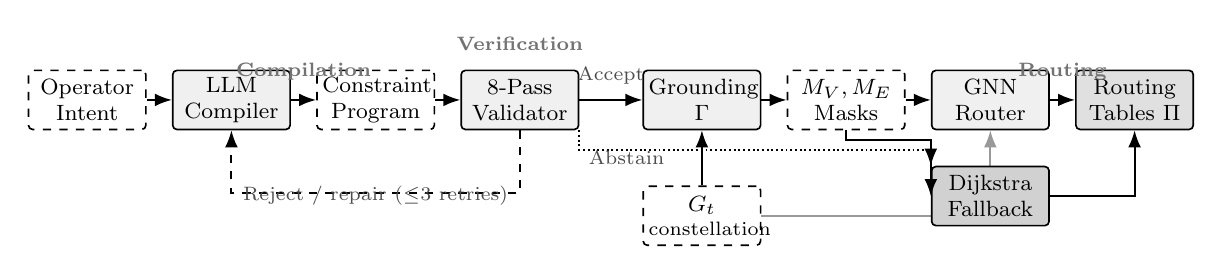
\begin{tikzpicture}[
    node distance=0.45cm and 0.32cm,
    box/.style={draw=black, rounded corners=1.5pt, line width=0.6pt,
                minimum height=0.75cm, text width=1.35cm,
                inner xsep=2pt, inner ysep=2pt,
                align=center, font=\footnotesize},
    comp/.style={box, fill=black!6},
    data/.style={box, fill=white, dashed},
    result/.style={box, fill=black!12},
    fallback/.style={box, fill=black!18},
    arr/.style={->, >=Latex, line width=0.7pt},
    reject/.style={arr, dashed},
    abstain/.style={arr, densely dotted},
    lbl/.style={font=\scriptsize, text=black!70},
]

% Main pipeline (single row)
\node[data] (intent) {Operator\\Intent};
\node[comp, right=of intent] (compiler) {LLM\\Compiler};
\node[data, right=of compiler] (ir) {Constraint\\Program};
\node[comp, right=of ir] (validator) {8-Pass\\Validator};
\node[comp, right=0.8cm of validator] (grounding) {Grounding\\$\Gamma$};
\node[data, right=of grounding] (masks) {$M_V, M_E$\\Masks};
\node[comp, right=of masks] (router) {GNN\\Router};
\node[result, right=of router] (routes) {Routing\\Tables $\Pi$};

% Main arrows
\draw[arr] (intent) -- (compiler);
\draw[arr] (compiler) -- (ir);
\draw[arr] (ir) -- (validator);

% Accept path (solid)
\draw[arr] (validator) -- (grounding);
\node[lbl, above=2pt] at ($(validator)!0.5!(grounding)$) {Accept};

\draw[arr] (grounding) -- (masks);
\draw[arr] (masks) -- (router);
\draw[arr] (router) -- (routes);

% Reject / Repair loop (dashed, below)
\draw[reject] (validator.south) -- ++(0,-0.8) -| (compiler.south);
\node[lbl] at ($(compiler.south)!0.5!(validator.south)+(0,-0.83)$)
  {Reject / repair ($\leq$3 retries)};

% Constellation graph input
\node[data, below=0.7cm of grounding] (graph) {$G_t$\\[-1pt]\scriptsize constellation};
\draw[arr] (graph) -- (grounding);
\draw[arr, black!40] (graph) -| (router);

% Dijkstra fallback (receives masked topology)
\node[fallback, below=0.45cm of router] (dijkstra) {Dijkstra\\Fallback};
\draw[arr] (masks.south) -- ++(0,-0.12) -| (dijkstra.west);
\draw[arr] (dijkstra) -| (routes.south);

% Abstain path (dotted, defers to Dijkstra)
\draw[abstain] (validator.south east) -- ++(0,-0.25) -| (dijkstra.north west);
\node[lbl] at ($(validator.south east)+(0.6,-0.35)$) {Abstain};

% Phase labels
\node[above=0.12cm of $(compiler)!0.5!(ir)$, font=\scriptsize\bfseries, text=black!55] {Compilation};
\node[above=0.12cm of validator, font=\scriptsize\bfseries, text=black!55] {Verification};
\node[above=0.12cm of $(router)!0.5!(routes)$, font=\scriptsize\bfseries, text=black!55] {Routing};

\end{tikzpicture}
\end{adjustbox}
\caption{End-to-end system architecture. Operator intents are compiled
to typed ConstraintPrograms and verified by the 8-pass validator.
Accept (solid) proceeds to grounding and GNN routing;
Reject (dashed) triggers repair; Abstain (dotted) defers to Dijkstra.}
\label{fig:system_architecture}
\end{figure*}


\subsection{Problem Formulation}
\label{sec:formulation}

We consider a Walker Delta constellation with $P$ orbital planes and
$S$ satellites per plane, yielding $N = P \times S$ nodes. This
configuration is representative of operational and planned
mega-constellations such as Starlink and OneWeb, which use similar
grid topologies at LEO altitudes~\cite{leo_constellation_survey}.
Each satellite maintains up to $K=4$ ISL links: two intra-plane links
connecting adjacent satellites within the same orbital plane, and two
inter-plane links connecting to the nearest satellites in neighboring
planes. Intra-plane ISLs are relatively stable because adjacent
satellites share similar orbital velocity and direction, making them
the backbone for along-track data forwarding. Inter-plane ISLs
connect satellites in different orbital planes with differing relative
motion, leading to higher beam-tracking complexity and periodic
dropout at high latitudes where orbital planes
converge~\cite{isl_dynamics}. This $K=4$ grid topology is the
standard model in the LEO routing
literature~\cite{snapshot_routing,drl_leo1}.

The constellation graph $G_t = (V, E_t)$ evolves over time as
satellite positions change and polar links experience periodic
dropout above inclination $\iota$. The system must support diverse
operational scenarios: remote sensing data relay with deadline
constraints, TT\&C traffic requiring protected low-latency paths,
and emergency rerouting during solar storms or equipment failures.

An operator intent $\ell$ is a natural language string expressing
routing constraints for such scenarios. For example, during a solar
storm an operator might issue: ``reroute all TT\&C traffic away from
polar links above 75\textdegree\ and guarantee latency under 80\,ms
for financial flows.'' The LEON pipeline processes this intent through
four stages:
\begin{enumerate}
\item \textit{Compile}: $\ell \xrightarrow{\text{LLM}} \mathcal{P}$,
mapping intent to a ConstraintProgram $\mathcal{P}$.
\item \textit{Verify}: $\mathcal{P} \xrightarrow{\text{Validator}}
\mathcal{P}^{\checkmark}$, ensuring structural and physical validity.
\item \textit{Ground}: $(\mathcal{P}^{\checkmark}, G_t)
\xrightarrow{\Gamma} (M_V, M_E, \mathbf{u}, \mathbf{d})$, producing
topology masks and flow constraints.
\item \textit{Route}: $(G_t \odot (M_V, M_E), \mathbf{d})
\xrightarrow{\text{GNN}} \Pi$, computing constrained routing tables.
\end{enumerate}

% Include formal IR definition
% ConstraintProgram IR Formal Definition
% For inclusion in paper Section III (System Design)

% Definition 1: ConstraintProgram
\begin{definition}[ConstraintProgram]
A \textit{ConstraintProgram} $\mathcal{P}$ is a typed intermediate representation
that captures operator intent as a tuple:
\begin{equation}
\mathcal{P} = \langle \mathcal{F}, \mathcal{H}, \mathcal{S}, \mathcal{E}, \omega, \pi \rangle
\end{equation}
where $\mathcal{F}$ is a set of flow selectors, $\mathcal{H}$ is a set of hard constraints,
$\mathcal{S}$ is a set of soft constraints, $\mathcal{E}$ is a set of event conditions,
$\omega$ is an objective weight vector, and $\pi \in \{\texttt{critical}, \texttt{high},
\texttt{medium}, \texttt{low}\}$ is the priority level.
\end{definition}

% Definition 2: Flow Selector
\begin{definition}[Flow Selector]
A flow selector $f \in \mathcal{F}$ identifies a subset of traffic flows:
\begin{equation}
f = \langle \tau, r_s, r_d, n_s, n_d, p_s, p_d \rangle
\end{equation}
where $\tau \in \mathcal{T}$ is a traffic class (e.g., \texttt{financial}, \texttt{emergency}),
$r_s, r_d \in \mathcal{R} \cup \{\bot\}$ are source/destination regions,
$n_s, n_d \in [0, N) \cup \{\bot\}$ are source/destination node IDs,
and $p_s, p_d \in [0, P) \cup \{\bot\}$ are source/destination orbital planes.
\end{definition}

% Definition 3: Hard Constraint
\begin{definition}[Hard Constraint]
A hard constraint $h \in \mathcal{H}$ must be satisfied; violation renders the
program infeasible:
\begin{equation}
h = \langle t_h, \sigma, v, c \rangle
\end{equation}
where $t_h \in \mathcal{T}_H$ is the constraint type, $\sigma$ is the target specifier,
$v$ is the constraint value, and $c \in \mathcal{E} \cup \{\bot\}$ is an optional
event condition.

The hard constraint type set is:
\begin{align}
\mathcal{T}_H = \{&\texttt{disable\_node}, \texttt{disable\_plane}, \texttt{disable\_edge}, \nonumber \\
                   &\texttt{avoid\_region}, \texttt{avoid\_latitude}, \texttt{reroute\_away}, \nonumber \\
                   &\texttt{max\_latency\_ms}, \texttt{max\_hops}, \nonumber \\
                   &\texttt{k\_edge\_disjoint}, \texttt{min\_capacity\_reserve}\}
\end{align}
\end{definition}

% Definition 4: Constraint Grounding
\begin{definition}[Constraint Grounding]
Given a constellation graph $G = (V, E)$ with $|V| = N$ nodes and topology
state at time $t$, the grounding function $\Gamma$ maps a ConstraintProgram
to topology modifications:
\begin{equation}
\Gamma(\mathcal{P}, G, t) = \langle M_V, M_E, \mathbf{u}, \mathbf{d} \rangle
\end{equation}
where $M_V \in \{0,1\}^N$ is a node mask, $M_E \in \{0,1\}^{|E|}$ is an edge mask,
$\mathbf{u} \in [0,1]^{|E|}$ is a per-edge utilization cap vector, and
$\mathbf{d}: \mathcal{F} \to \mathbb{R}^+$ maps flow selectors to deadline values.

Grounding rules for topology-modifying constraints:
\begin{itemize}
\item $\texttt{disable\_node}(n)$: $M_V[n] \leftarrow 0$, propagate to incident edges
\item $\texttt{disable\_plane}(p)$: $\forall s \in [0, S): M_V[p \cdot S + s] \leftarrow 0$
\item $\texttt{avoid\_latitude}(\theta)$: $\forall (u,v) \in E: |\phi_u| > \theta \lor |\phi_v| > \theta \Rightarrow M_E[(u,v)] \leftarrow 0$
\item $\texttt{avoid\_region}(r)$: $\forall (u,v) \in E: u \in \mathcal{N}_r \lor v \in \mathcal{N}_r \Rightarrow M_E[(u,v)] \leftarrow 0$
\end{itemize}
where $\phi_n$ is the latitude of node $n$ and $\mathcal{N}_r$ is the set of nodes
within region $r$.
\end{definition}

% Table: Constraint Types and Grounding Semantics
\begin{table}[t]
\centering
\caption{ConstraintProgram hard constraint types and their grounding semantics.}
\label{tab:constraint_types}
\begin{tabular}{lll}
\toprule
\textbf{Type} & \textbf{Target} & \textbf{Grounding} \\
\midrule
\texttt{disable\_node} & \texttt{node:$n$} & $M_V[n] \leftarrow 0$ \\
\texttt{disable\_plane} & \texttt{plane:$p$} & $M_V[pS{:}(p{+}1)S] \leftarrow 0$ \\
\texttt{avoid\_latitude} & \texttt{edges:ALL} & $M_E[(u,v)] \leftarrow 0$ if $|\phi| > \theta$ \\
\texttt{avoid\_region} & \texttt{region:$r$} & $M_E[(u,v)] \leftarrow 0$ if $u,v \in \mathcal{N}_r$ \\
\texttt{reroute\_away} & \texttt{node:$n$} & $M_V[n] \leftarrow 0$ (transit) \\
\texttt{max\_latency\_ms} & \texttt{flow\_sel:$i$} & $\mathbf{d}[f_i] \leftarrow v$ \\
\texttt{max\_hops} & \texttt{flow\_sel:$i$} & hop limit on path \\
\bottomrule
\end{tabular}
\end{table}


\subsection{GNN Cost-to-Go Router}
\label{sec:gnn_router}

The routing component must compute next-hop decisions for all
origin-destination pairs on the (possibly constrained) topology graph.
We train a GNN to approximate Dijkstra's cost-to-go function via
supervised distillation.

\subsubsection{Architecture}
The encoder is a 3-layer Graph Attention Network (GAT)~\cite{gat}
with 128-dimensional hidden states and 4 attention heads per layer.
Input node features $\mathbf{x}_i \in \mathbb{R}^{10}$ encode:
satellite position (latitude, longitude, altitude), orbital parameters
(plane ID, slot ID as sinusoidal encodings), and local topology
statistics (degree, mean neighbor delay).

For each destination $d$, the scorer computes a cost-to-go estimate
for each neighbor $j$ of node $i$:
\begin{equation}
\hat{c}(i, j, d) = \text{MLP}\big([\mathbf{h}_i \| \mathbf{h}_j \|
\mathbf{h}_d \| \mathbf{e}_{ij}]\big)
\end{equation}
where $\mathbf{h}_i$ is the GAT embedding of node $i$, $\|$ denotes
concatenation, and $\mathbf{e}_{ij}$ encodes edge features (delay,
capacity). The next hop is $\arg\min_j \hat{c}(i, j, d)$.

\subsubsection{Training}
We generate 500 topology snapshots by sampling constellation states
at random orbital phases. For each snapshot, Dijkstra's algorithm
computes the optimal next-hop table $\Pi^* \in [K]^{N \times N}$.
The model is trained for 200 epochs with cross-entropy loss on
next-hop predictions, using a phased curriculum: 50 epochs on
easy pairs (hop distance $\leq 5$), then 150 epochs on all pairs.

\subsubsection{Constrained Routing}
When constraints are active, the grounding function $\Gamma$ produces
node mask $M_V$ and edge mask $M_E$. The constrained graph
$G' = (V \odot M_V, E \odot M_E)$ is passed to the GNN, which
computes routing tables on the reduced topology. This approach
requires no retraining---the GNN generalizes to unseen topologies
through its message-passing architecture.

\subsection{LLM Intent Compiler}
\label{sec:compiler}

The compiler translates natural language intents to ConstraintProgram
JSON using a three-stage pipeline: few-shot prompting, JSON extraction,
and verifier-feedback repair.

\subsubsection{Prompt Design}
The system prompt (approximately 800 tokens) specifies the constellation
parameters, the complete ConstraintProgram JSON schema, all valid enum
values, target format conventions, and 6 compilation rules. Five
in-context examples cover single constraints (node disable, latency
SLA), compositional constraints (plane disable + polar avoidance +
utilization cap), and conditional constraints (event-triggered reroute).

\subsubsection{Repair Loop}
When the verifier rejects a compiled program, the error messages are
appended to the conversation as a repair prompt. The compiler retries
up to 3 total attempts (1 initial + 2 repairs), with each attempt receiving the accumulated error
context. This closed-loop design converts verifier precision into
compiler accuracy: under uniform random edge delays, 93.3\% of all
240 intents compile on the first attempt, and the repair loop raises
this to 97.9\% (+4.6pp). Under distance-based ISL delays, first-attempt
accuracy drops to 77.9\%, with repair raising it to 85.0\% (+7.1pp).

\subsubsection{JSON Extraction}
The extractor handles three response formats: raw JSON, markdown-fenced
JSON, and JSON embedded in explanatory text. It also strips reasoning
tags (\texttt{<think>}) produced by instruction-tuned models. Robust
extraction is critical because even high-quality LLMs occasionally
wrap JSON in commentary.

% Include validator design
% Validator Design Rationale Subsection
% For inclusion in paper Section III-C (Deterministic Validation Pipeline)

\subsection{Deterministic Validation Pipeline}
\label{sec:validator}

A key design principle of our system is that the LLM compiler operates
\textit{offline} and its output is never trusted directly. Every
ConstraintProgram passes through an 8-pass deterministic validator before
reaching the routing layer. This design is motivated by two observations:
(1)~LLMs can produce syntactically valid but semantically incorrect
constraint programs, and (2)~in safety-critical network infrastructure,
a single undetected constraint violation can cascade into service outages.

The validator implements the following passes in sequence, with early
termination on fatal errors:

\begin{enumerate}
\item \textbf{Schema Validation.} Checks structural completeness: all
required fields present, valid priority levels, non-empty constraint
types and targets. Rejects malformed programs before deeper analysis.

\item \textbf{Entity Grounding.} Verifies that all referenced entities
exist in the constellation model: node IDs $\in [0, N)$, plane IDs
$\in [0, P)$, region names $\in \mathcal{R}$, traffic classes
$\in \mathcal{T}$. This catches hallucinated entities (e.g., node~454
in a 400-node constellation).

\item \textbf{Type Safety.} Ensures constraints attach to semantically
correct entity types: \texttt{max\_latency\_ms} must target a
\texttt{flow\_selector}, \texttt{disable\_node} must target a
\texttt{node}, \texttt{avoid\_latitude} must target \texttt{edges}.
Prevents type confusion errors where the LLM assigns a constraint
to the wrong entity class.

\item \textbf{Value Range Checking.} Validates numeric parameters:
latitudes $\in [-90, 90]$, latency values $> 0$, utilization caps
$\in (0, 1]$, node IDs within constellation bounds. Catches
out-of-range values that would produce undefined behavior.

\item \textbf{Conflict Detection.} Identifies contradictory constraints
within the same program: a node cannot be simultaneously disabled and
used as a routing waypoint; conflicting latency bounds on the same flow
are flagged. Contradictions are promoted to errors (not warnings),
ensuring logically inconsistent programs are rejected.

\item \textbf{Physical Admissibility.} Checks whether the constrained
topology is physically realizable: latency deadlines below the
single-hop physical minimum ($<2.0$\,ms) are rejected; latitude
avoidance thresholds that remove $>50\%$ of edges trigger warnings.

\item \textbf{Reachability Analysis.} Performs BFS on the constrained
graph $G' = (V \odot M_V, E \odot M_E)$ to verify connectivity.
Severe capacity loss ($\geq 75\%$ of nodes disabled) triggers a strong
warning; moderate loss ($\geq 50\%$) triggers a standard warning.
These capacity thresholds are heuristic indicators outside the
soundness path---they do not block acceptance, which is determined
solely by Pass~8.

\item \textbf{Feasibility Certification.} For each demanded flow,
constructs a routing witness on the constrained topology to certify
that all hard constraints can be simultaneously satisfied. Five
certified fragments cover the constraint space:
\begin{itemize}
\item \textbf{F1} (topology only): BFS reachability
\item \textbf{F2} (+ latency): Dijkstra with deadline
\item \textbf{F3} (+ hops): BFS with hop limit
\item \textbf{F4} (+ latency + hops): hop-layered Dijkstra
\item \textbf{F5} (+ $k$-disjoint): Edmonds-Karp max-flow
\end{itemize}
Three outcomes: \decision{accept} (witness found), \decision{reject}
(no feasible routing exists), or \decision{abstain} (unsupported
constraint combination). Programs are rejected only on \decision{reject};
\decision{abstain} defers to Dijkstra fallback routing, preserving
safety without constructive certification.
\end{enumerate}

\begin{theorem}[Acceptance Soundness]
If the feasibility certifier accepts a constraint program $P$ with
witness $W$, then there exists a routing assignment satisfying all
hard constraints of $P$ on the constrained topology.
\end{theorem}

\begin{proof}[Proof sketch]
By case analysis over fragments F1--F5. Each fragment's algorithm
is a standard shortest-path or max-flow algorithm whose correctness
is well-established. The witness $W$ is the concrete path (or path set)
returned by the algorithm, which by construction satisfies the
topology constraints (disabled nodes/edges excluded from the search
graph), latency bounds (Dijkstra optimality), hop limits (BFS layering),
and disjointness requirements (augmenting path decomposition).
Unsupported combinations produce \decision{abstain}, never
\decision{accept}, so no false acceptance is possible within the
certified fragment space.
\end{proof}

\noindent\textbf{Design rationale.} We chose deterministic
validation over learned or probabilistic checking for three reasons:
\begin{itemize}
\item \textit{Completeness}: every structural error class is covered by
at least one pass, achieving 100\% detection on our corruption benchmark
(8 error types $\times$ 30 injections = 240 tests).
\item \textit{Transparency}: each rejection includes a human-readable
error message identifying the specific violation, enabling the repair
loop to provide targeted feedback to the LLM.
\item \textit{Soundness}: the feasibility certifier guarantees that
accepted programs have constructive routing witnesses, closing the
semantic gap between structural validity and routing feasibility.
\end{itemize}

\noindent\textbf{Repair loop integration.} When validation fails, the
error messages are fed back to the LLM as a repair prompt. The compiler
retries up to $k=3$ times, with each attempt receiving the previous
errors as context. In our 240-benchmark evaluation (uniform random edge delays), 97.9\% of intents
compile successfully, with 93.3\% succeeding on the first attempt.


% Validator pipeline figure
% Validator Pipeline Figure (TikZ)
% Single-column figure for inclusion in paper_main.tex

\begin{figure}[t]
\centering
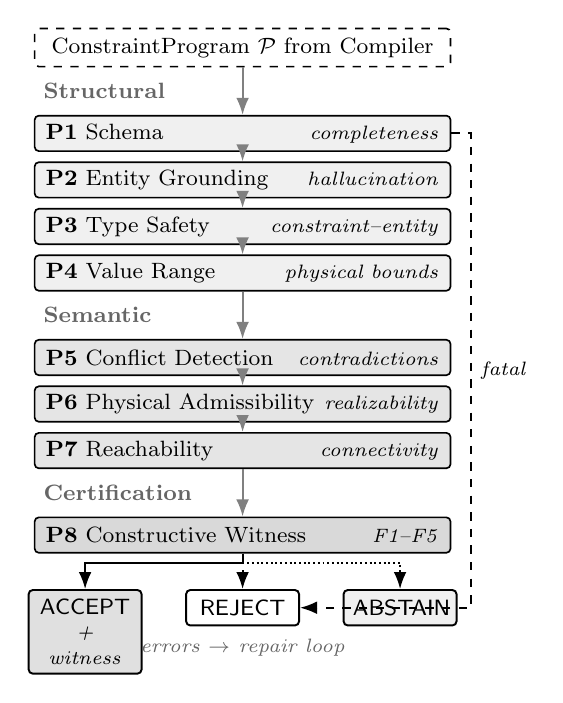
\begin{tikzpicture}[
    node distance=0.15cm,
    pass/.style={draw=black, rounded corners=1.5pt, line width=0.6pt,
                 minimum height=0.45cm, text width=5.0cm,
                 inner xsep=4pt, inner ysep=2pt,
                 align=left, font=\footnotesize, fill=black!6},
    group/.style={font=\footnotesize\bfseries, text=black!60},
    outcome/.style={draw=black, rounded corners=1.5pt, line width=0.7pt,
                    minimum height=0.45cm, text width=1.2cm,
                    align=center, font=\footnotesize},
    arr/.style={->, >=Latex, line width=0.7pt, black!50},
    fatal/.style={->, >=Latex, line width=0.7pt, dashed},
]

% Input
\node[draw=black, dashed, rounded corners=1.5pt, line width=0.6pt,
      minimum height=0.45cm, text width=5.0cm, fill=white,
      font=\footnotesize, align=center, inner xsep=4pt]
      (input) {ConstraintProgram $\mathcal{P}$ from Compiler};

% Structural checks group
\node[group, below=0.3cm of input.south west, anchor=west] (g1) {Structural};
\node[pass, below=0.08cm of g1.south west, anchor=north west] (p1)
     {\textbf{P1} Schema \hfill \textit{\scriptsize completeness}};
\node[pass, below=0.12cm of p1] (p2)
     {\textbf{P2} Entity Grounding \hfill \textit{\scriptsize hallucination}};
\node[pass, below=0.12cm of p2] (p3)
     {\textbf{P3} Type Safety \hfill \textit{\scriptsize constraint--entity}};
\node[pass, below=0.12cm of p3] (p4)
     {\textbf{P4} Value Range \hfill \textit{\scriptsize physical bounds}};

% Semantic checks group
\node[group, below=0.3cm of p4.south west, anchor=west] (g2) {Semantic};
\node[pass, below=0.08cm of g2.south west, anchor=north west, fill=black!10] (p5)
     {\textbf{P5} Conflict Detection \hfill \textit{\scriptsize contradictions}};
\node[pass, below=0.12cm of p5, fill=black!10] (p6)
     {\textbf{P6} Physical Admissibility \hfill \textit{\scriptsize realizability}};
\node[pass, below=0.12cm of p6, fill=black!10] (p7)
     {\textbf{P7} Reachability \hfill \textit{\scriptsize connectivity}};

% Feasibility certification
\node[group, below=0.3cm of p7.south west, anchor=west] (g3) {Certification};
\node[pass, below=0.08cm of g3.south west, anchor=north west, fill=black!15] (p8)
     {\textbf{P8} Constructive Witness \hfill \textit{\scriptsize F1--F5}};

% Arrows between passes
\foreach \a/\b in {input/p1, p1/p2, p2/p3, p3/p4, p4/p5, p5/p6, p6/p7, p7/p8} {
    \draw[arr] (\a) -- (\b);
}

% Three outcomes
\node[outcome, below=0.45cm of p8, xshift=-2.0cm, fill=black!12]
     (accept) {\decision{Accept}\\[-1pt]\scriptsize\textit{+ witness}};
\node[outcome, below=0.45cm of p8, fill=white]
     (reject) {\decision{Reject}};
\node[outcome, below=0.45cm of p8, xshift=2.0cm, fill=black!6]
     (abstain) {\decision{Abstain}};

% Outcome arrows with line style differentiation
\draw[->, >=Latex, line width=0.7pt] (p8.south) -- ++(0,-0.12) -| (accept);
\draw[->, >=Latex, line width=0.7pt, dashed] (p8.south) -- (reject);
\draw[->, >=Latex, line width=0.7pt, densely dotted] (p8.south) -- ++(0,-0.12) -| (abstain);

% Early termination arrow
\draw[fatal] (p1.east) -- ++(0.25,0) |- node[font=\scriptsize\itshape, near start, right] {fatal} (reject.east);

% Repair loop annotation
\node[font=\scriptsize\itshape, text=black!60, below=0.04cm of reject]
     {errors $\to$ repair loop};

\end{tikzpicture}
\caption{8-pass validation pipeline. Passes 1--4 check structural
validity; 5--7 check semantic consistency; Pass~8 constructs routing
witnesses (BFS, Dijkstra, Edmonds-Karp). Solid/dashed/dotted arrows
indicate Accept/Reject/Abstain outcomes.}
\label{fig:validator_pipeline}
\end{figure}


% Include infeasible handling
% Infeasible Intent Handling and Fallback Policies
% For inclusion in paper Section III-D or IV (Discussion)

\subsection{Handling Infeasible, Ambiguous, and Edge-Case Intents}
\label{sec:infeasible_handling}

Real-world operator intents are not always well-formed or physically
realizable. Our system addresses three categories of problematic intents
through complementary mechanisms.

\subsubsection{Infeasible Intent Detection}

An intent is \textit{infeasible} when its constraint program is
syntactically valid but physically unrealizable---e.g., demanding
sub-millisecond latency across intercontinental paths, or routing through
a region after disabling all nodes in that region. Our 8-pass validator
detects three classes of infeasibility:

\begin{itemize}
\item \textbf{Structural infeasibility} (100\% detection): missing fields,
out-of-range entity IDs, type mismatches, and values outside physical
bounds (e.g., latency $< 2.0$\,ms). These are caught by passes 1--4
(schema, entity grounding, type safety, value ranges).

\item \textbf{Topological infeasibility} (100\% detection): constraints
that partition the network, eliminate viable paths, or cause severe
capacity loss. Pass~5 rejects contradictory constraints (e.g., disabling
a node while routing through it). Pass~7 warns when $\geq 50\%$ of nodes are disabled (severe capacity
loss) and escalates to a stronger warning at $\geq 75\%$. These
capacity thresholds are heuristic warnings outside the soundness
path---they do not block acceptance.

\item \textbf{Routing infeasibility} (100\% detection within certified
fragments): constraint combinations that are individually valid but
jointly unsatisfiable on the physical topology. Pass~8 (feasibility
certification) constructs routing witnesses using fragment-specific
algorithms (BFS, Dijkstra, hop-layered Dijkstra, Edmonds-Karp max-flow)
and rejects programs where no witness exists.
\end{itemize}

\noindent Our confusion matrix (Table~\ref{tab:confusion_matrix})
confirms the effectiveness of the 8-pass pipeline: 0\% unsafe acceptance
across all categories. Of the 30 benchmark-infeasible intents, 22 receive
\decision{Reject} and 8 receive \decision{Abstain}---none are accepted.
Pass~8 additionally identifies 32 programs among the structurally-valid
set whose latency or hop constraints cannot be satisfied on the physical
constellation topology (e.g., 30\,ms S\~{a}o Paulo--New York when the
minimum-hop path requires $\sim$63\,ms); 29/32 are independently
confirmed via a separate Dijkstra oracle.

Our adversarial safety evaluation (15 tests across resource exhaustion,
semantic conflicts, and boundary exploitation) achieves 100\% detection
(15/15), including near-total capacity removal (disabling 19/20 planes),
cross-constraint contradictions, and boundary value exploitation.

\subsubsection{Fallback Policies}

The ConstraintProgram IR includes a \texttt{fallback\_policy} field that
governs system behavior when hard constraints cannot be satisfied at
routing time:

\begin{enumerate}
\item \texttt{reject\_if\_hard\_infeasible} (default): the routing layer
refuses to compute paths and returns an explicit failure to the operator.
This is the safest option for critical intents where partial compliance
is unacceptable.

\item \texttt{relax\_soft\_first}: soft constraints are progressively
relaxed (in order of increasing penalty weight) until a feasible routing
exists. Hard constraints are never relaxed. This enables graceful
degradation for intents where approximate compliance is preferable to
total failure.

\item \texttt{report\_unsat\_core}: the system identifies the minimal
subset of constraints that cause infeasibility and reports them to the
operator, enabling informed manual intervention. This supports
diagnostic workflows where understanding \textit{why} an intent fails
is as important as resolving it.
\end{enumerate}

\noindent In our 240-intent benchmark, all programs use the default
\texttt{reject\_if\_hard\_infeasible} policy. The fallback mechanism
is designed for operational deployment where operator interaction is
available; evaluating its effectiveness under dynamic network conditions
is left to future work.

\subsubsection{Ambiguous Intent Resolution}

Ambiguous intents admit multiple valid interpretations. Our OOD
evaluation includes 5 deliberately ambiguous intents (e.g., ``optimize
the network for best performance'') to assess compiler behavior.
Key observations:

\begin{itemize}
\item The LLM compiler produces \textit{reasonable} constraint programs
for all 5 ambiguous intents (qualitative assessment), typically selecting
conservative interpretations that map to load-balancing or latency
optimization.

\item Ambiguous intents are excluded from quantitative scoring because
no unique ground truth exists. We report them separately as qualitative
evidence of graceful degradation.

\item The compiler's 6-shot prompt includes examples that implicitly
demonstrate disambiguation strategies (e.g., mapping vague performance
requests to specific constraint types), providing soft guidance without
explicit disambiguation rules.
\end{itemize}

\subsubsection{Limitations and Future Directions}

The feasibility certifier covers five constraint fragments (F1--F5)
that span the most common constraint combinations in our benchmark.
Three directions could extend coverage further:

\begin{enumerate}
\item \textbf{Extended fragment coverage}: constraints involving
\texttt{min\_cap\_reserve} or combinations of $k$-disjoint paths
with latency/hop bounds currently produce \decision{Abstain}. Adding
fragments for these combinations (e.g., via constrained max-flow)
would reduce the abstain rate.

\item \textbf{Multi-constellation generalization}: cross-constellation
evaluation (Table~\ref{tab:cross_constellation}) shows the GNN
generalizes to altitude changes but not inclination changes.
The compile--verify--ground pipeline is constellation-agnostic,
but the GNN requires retraining per orbital geometry. Extending
to heterogeneous multi-shell constellations (e.g., Starlink Gen2)
remains future work.

\item \textbf{Intent confirmation loop}: presenting the grounded
constraint program back to the operator in natural language for
confirmation before execution, closing the semantic loop between
intent and realization.
\end{enumerate}


% ============================================================
\section{Evaluation}
\label{sec:eval}

The evaluation is designed to answer four questions, each corresponding
to a core claim of LEON. (1)~Does the GNN router match Dijkstra
quality while providing meaningful speedup for real-time constrained
routing? (2)~Does the LLM compiler accurately translate compositional
operator intents, and how much does each pipeline component
contribute? (3)~Does the 8-pass validator reliably block unsafe or
infeasible intents (via \decision{Reject} or \decision{Abstain})
before they reach the routing layer? (4)~Does the
full LEON pipeline maintain zero constraint violations across
constrained scenarios including node failure, plane maintenance,
polar avoidance, and compositional constraints?
The results confirm that the GNN matches Dijkstra PDR within
measurement noise, the compiler substantially outperforms rule-based
parsing on compositional intents, the validator achieves 0\% unsafe
acceptance, and the end-to-end pipeline produces no constraint
violations across all tested scenarios.

All experiments run on a single workstation with an Intel Core Ultra~9
185H CPU (16\,GB RAM) and NVIDIA RTX 4060 GPU (8\,GB VRAM) under
Ubuntu 24.04. The LLM compiler runs locally via LM Studio; no cloud
API is required.

\subsection{Experimental Setup}
\label{sec:setup}

\textbf{Constellation.} Walker Delta 20$\times$20 (400 nodes, 550\,km
altitude, 53\textdegree\ inclination), 4 grid ISL neighbors per
satellite. Topology snapshots sampled at random orbital phases.

\textbf{GNN Router.} 3-layer GAT encoder (128-dim, 4 heads), MLP
cost-to-go scorer (rank 64). 152,193 parameters. Trained 200 epochs
on 500 snapshots. Hardware: NVIDIA RTX 4060 (8\,GB VRAM).

\textbf{LLM Compiler.} Qwen3.5-9B (GGUF quantization) served locally
via LM Studio. Temperature 0.1, max 2048 tokens, up to 3 total
attempts (1 initial + 2 repairs). 5-shot prompt (5 examples spanning single, compositional,
and conditional categories).

\textbf{Benchmark.} 240 intents by category: 80 single-constraint,
100 compositional (2--4 constraints), 30 conditional (event-triggered),
30 labeled-infeasible (physically unrealizable). Each intent has a
ground-truth ConstraintProgram for automated scoring. All compiler
comparison and ablation tables use uniform random edge delays over
all 240 intents. A separate distance-based ISL delay rerun (9B only;
which also uses a slightly different coordinate discretization,
endpoint-exclusive rather than endpoint-inclusive) yields 85.0\% compiled and 70.4\% full
match over all 240 intents; the drop from 86.2\% reflects both the
harder delay model and the discretization change, and the two effects
are not isolated in this rerun.
Safety metrics (unsafe acceptance) always use all 240 intents.

\textbf{Metrics.} \textit{Compiled}: produces a ConstraintProgram that
is not rejected by the full 8-pass validator (includes both
\decision{Accept} and \decision{Abstain}; excludes \decision{Reject}).
\textit{Unsafe acceptance}: a labeled-infeasible intent receiving
\decision{Accept}; \decision{Abstain} is treated as safe fallback,
not acceptance.
\textit{Types match}: correct constraint type multiset.
\textit{Full match}: types + targets + values match (primary metric).
\textit{PDR}: packet delivery ratio over 100 random OD pairs $\times$
50 time steps $\times$ 3 seeds.

\subsection{GNN Routing Performance}
\label{sec:eval_gnn}

Table~\ref{tab:gnn_baseline} summarizes GNN routing quality across
five traffic scenarios without constraints.

\begin{table}[t]
\centering
\caption{GNN cost-to-go routing vs.\ Dijkstra baseline (unconstrained).}
\label{tab:gnn_baseline}
\begin{tabular}{lccc}
\toprule
\textbf{Scenario} & \textbf{GNN PDR} & \textbf{Dijkstra PDR} & \textbf{Random PDR} \\
\midrule
Uniform    & 99.75\% & 99.75\% & 0.90\% \\
Hotspot    & 99.99\% & 99.99\% & 2.36\% \\
Regional   & 99.94\% & 99.94\% & 5.49\% \\
Polar      & 100.0\% & 100.0\% & 1.88\% \\
Flash      & 99.77\% & 99.77\% & 0.89\% \\
\bottomrule
\end{tabular}
\end{table}

The GNN matches Dijkstra within measurement noise across all scenarios,
confirming successful distillation. Detailed metrics on 10 snapshots
show 95.8\% exact next-hop match, zero routing loops, hop stretch of
1.000, and P99 delay stretch of 1.015. Inference latency is 8.4\,ms
(GNN) vs.\ 142\,ms (Dijkstra), a 17$\times$ speedup.

\subsection{Intent Compilation Accuracy}
\label{sec:eval_compiler}

\subsubsection{Ablation Study}

Table~\ref{tab:ablation} presents the ablation study across four
compiler configurations on the full 240-intent benchmark. All ablation
and comparison tables use uniform random edge delays for controlled
comparison across configurations. A separate distance-based ISL delay rerun
(9B only; see Section~\ref{sec:setup} for the coordinate discretization note)
yields 85.0\% compiled and 70.4\% full match over all 240 intents;
the two confounds (delay model and discretization) are not isolated.

\begin{table}[t]
\centering
\caption{Compiler ablation study (240 intents, uniform random edge delays).}
\label{tab:ablation}
\begin{tabular}{lcccc}
\toprule
\textbf{Config} & \textbf{Compiled} & \textbf{Types} & \textbf{Full Match} & \textbf{Latency} \\
\midrule
Full pipeline  & 97.9\% & 91.7\% & \textbf{86.2\%} & 15.7s \\
No verifier    & 100.0\% & 93.8\% & 91.7\% & 13.8s \\
No repair      & 92.9\% & 86.7\% & 84.6\% & 13.8s \\
Zero-shot      & 92.5\% & 71.7\% & 15.4\% & 34.2s \\
\bottomrule
\end{tabular}
\end{table}

Few-shot prompting is the dominant factor: removing it (zero-shot)
drops full match from 86.2\% to 15.4\% ($-$70.8pp). The repair loop
contributes 5.0pp to compilation rate and 1.6pp to full match. The
``no verifier'' configuration shows higher apparent accuracy because
unverified programs are not filtered---a misleading metric that
underscores the importance of verification.

% Include compiler comparison and other tables
% Paper Tables: New experimental results
% Confusion Matrix, Reachability Separation, Compiler Comparison,
% Cross-Constellation, Polar Exclusion, Runtime Benchmark

% ============================================================
% Table: Verifier Confusion Matrix (3-way)
% ============================================================
\begin{table}[t]
\centering
\caption{Three-way validator confusion matrix on the 240-intent benchmark
(8-pass pipeline with constructive feasibility certification).
\textsc{Accept} requires a routing witness; \textsc{Abstain} indicates
unsupported constraint combinations (safe non-accept). The validator
achieves 0\% unsafe acceptance across all categories.}
\label{tab:confusion_matrix}
\begin{tabular}{lccc}
\toprule
& \textbf{Accept} & \textbf{Reject} & \textbf{Abstain} \\
\midrule
Single ($n$=80)         & 10  & 5   & 65  \\
Compositional ($n$=100) & 40  & 25  & 35  \\
Conditional ($n$=30)    & 8   & 2   & 20  \\
Infeasible ($n$=30)     & 0   & 22  & 8   \\
\midrule
\textbf{Total} ($n$=240) & 58 & 54 & 128 \\
\midrule
\multicolumn{4}{l}{\textit{Safety (unsafe = infeasible \textsc{Accept}):}} \\
\quad Infeasible       & \multicolumn{3}{l}{0/30 = 0\% (was 72\% with 7-pass)} \\
\multicolumn{4}{l}{\textit{Coverage (\textsc{Accept}+\textsc{Reject}):}} \\
\quad Decided          & \multicolumn{3}{l}{112/240 = 46.7\%} \\
\bottomrule
\multicolumn{4}{l}{\footnotesize 32 feasible programs rejected as routing-infeasible;} \\
\multicolumn{4}{l}{\footnotesize 29/32 independently confirmed via separate Dijkstra oracle.} \\
\end{tabular}
\end{table}

% ============================================================
% Table: Reachability Separation
% ============================================================
\begin{table}[t]
\centering
\caption{Reachability separation analysis. Raw PDR differences in
polar/compositional scenarios are entirely explained by the reachability
ceiling (76\% of OD pairs unreachable), not routing quality. Both GNN
and Dijkstra achieve 100\% delivery on reachable pairs.}
\label{tab:reachability}
\begin{tabular}{lccccc}
\toprule
\textbf{Scenario} & \textbf{Reach.} & \multicolumn{2}{c}{\textbf{Raw PDR}} & \multicolumn{2}{c}{\textbf{Reachable PDR}} \\
\cmidrule(lr){3-4} \cmidrule(lr){5-6}
& & GNN & Dijkstra & GNN & Dijkstra \\
\midrule
Baseline          & 100\%  & 99.8\% & ---     & 99.8\% & ---     \\
Node failure      & 100\%  & 98.7\% & 97.8\%  & 98.7\% & 97.8\% \\
Plane maint.      & 100\%  & 70.5\% & 70.2\%  & 70.5\% & 70.2\% \\
Polar avoid.      & 24.0\% & 34.6\% & 47.9\%  & 100\%  & 100\%  \\
Compositional     & 24.0\% & 34.3\% & 47.1\%  & 100\%  & 100\%  \\
\bottomrule
\end{tabular}
\end{table}

% ============================================================
% Table: Compiler Comparison (Rule-Based vs LLM)
% ============================================================
\begin{table}[t]
\centering
\caption{Intent compiler comparison on the 240-intent benchmark
(193 feasible intents; 17 additional routing-infeasible discovered
by Pass~8 excluded from feasible metrics).
The rule-based parser handles simple intents adequately but degrades
sharply on compositional intents, confirming that intent compilation
is a compositional reasoning task that benefits from LLM capabilities.}
\label{tab:compiler_comparison}
\begin{tabular}{lccc}
\toprule
\textbf{Metric} & \textbf{Rule-Based} & \textbf{LLM 4B} & \textbf{LLM 9B} \\
\midrule
Compiled          & 100.0\% & 59.6\% & \textbf{98.4\%} \\
Types Match       & 67.1\%  & 55.4\% & \textbf{91.7\%} \\
Full Match        & 56.7\%  & 54.2\% & \textbf{87.6\%} \\
Avg Latency       & \textbf{0.05ms} & 204s & 15.7s \\
\midrule
\multicolumn{4}{l}{\textit{Full match by category:}} \\
\quad Single      & 76.2\%  & ---    & \textbf{89.5\%} \\
\quad Compositional & 40.0\% & ---   & \textbf{86.2\%} \\
\quad Conditional & 66.7\%  & ---    & \textbf{86.7\%} \\
\quad Infeasible  & 50.0\%  & ---    & \textbf{73.3\%} \\
\bottomrule
\end{tabular}
\end{table}

% ============================================================
% Table: OOD Generalization
% ============================================================
\begin{table}[t]
\centering
\caption{Out-of-distribution generalization on paraphrased intents
(38 total: 33 scorable + 5 ambiguous). The compiler maintains 81.8\%
full match accuracy with only 4.4pp degradation from template intents,
demonstrating robust generalization to novel phrasings.}
\label{tab:ood}
\begin{tabular}{lccc}
\toprule
\textbf{Category} & \textbf{N} & \textbf{Compiled} & \textbf{Full Match} \\
\midrule
Single         & 20 & 100\% & 95.0\% (19/20) \\
Compositional  & 5  & 100\% & 40.0\% (2/5)   \\
Conditional    & 8  & 100\% & 75.0\% (6/8)   \\
Ambiguous      & 5  & 100\% & qualitative: 5/5 \\
\midrule
Scorable total & 33 & 100\% & \textbf{81.8\%} (27/33) \\
\bottomrule
\end{tabular}
\end{table}

% ============================================================
% Table: Cross-Model Scaling (4B vs 9B)
% ============================================================
\begin{table}[t]
\centering
\caption{Cross-model scaling: 4B vs 9B parameter LLM on the full
240-intent benchmark. The 9B model dramatically outperforms the 4B
model, suggesting a compositional complexity threshold between 4B
and 9B parameters for this task.}
\label{tab:cross_model}
\begin{tabular}{lcc}
\toprule
\textbf{Metric} & \textbf{Qwen 4B} & \textbf{Qwen 9B} \\
\midrule
Compiled       & 59.6\% & \textbf{98.4\%} \\
Types Match    & 55.4\% & \textbf{91.7\%} \\
Full Match     & 54.2\% & \textbf{87.6\%} \\
First-try Rate & 47.1\% & \textbf{89.2\%} \\
Avg Latency    & 204.4s & \textbf{15.7s}  \\
\bottomrule
\end{tabular}
\end{table}

% ============================================================
% Table: Topology Sweep (GNN vs Dijkstra across severity)
% ============================================================
\begin{table}[t]
\centering
\caption{GNN vs Dijkstra PDR across topology degradation severity
(orbital plane removal, 20 sats/plane). The GNN router matches
Dijkstra within 0.22pp at all severity levels, confirming robust
distillation quality. Non-monotonic PDR reflects topology-dependent
reachability under random plane selection (3-seed average).}
\label{tab:topology_sweep}
\begin{tabular}{rrccc}
\toprule
\textbf{Planes Off} & \textbf{Capacity} & \textbf{GNN PDR} & \textbf{Dijkstra PDR} & \textbf{$\Delta$} \\
\midrule
1  & 5\%  & 81.1\% & 80.9\% & +0.22 \\
2  & 10\% & 41.1\% & 41.1\% & 0.00 \\
3  & 15\% & 36.8\% & 36.8\% & 0.00 \\
5  & 25\% & 45.3\% & 45.3\% & 0.00 \\
7  & 35\% & 42.5\% & 42.5\% & 0.00 \\
10 & 50\% & 11.4\% & 11.4\% & 0.00 \\
13 & 65\% & 5.4\%  & 5.4\%  & 0.00 \\
15 & 75\% & 5.5\%  & 5.5\%  & 0.00 \\
17 & 85\% & 36.4\% & 36.4\% & 0.00 \\
\bottomrule
\end{tabular}
\end{table}

% ============================================================
% Table: Cross-Constellation GNN Generalization
% ============================================================
\begin{table}[t]
\centering
\caption{Zero-shot cross-constellation GNN generalization. The GNN
(trained on Walker Delta 550\,km/53$^\circ$) generalizes perfectly to
altitude changes (same grid topology, different edge weights) but
collapses on SSO 97$^\circ$ where near-polar inclination fundamentally
alters ISL geometry. This motivates the compile--verify--ground pipeline
as the constellation-agnostic safety layer, with the GNN as a fast
accelerator for a specific configuration.}
\label{tab:cross_constellation}
\begin{tabular}{lccc}
\toprule
\textbf{Configuration} & \textbf{GNN PDR} & \textbf{Dijkstra PDR} & \textbf{$\Delta$} \\
\midrule
550\,km / 53$^\circ$ (training) & 99.75\% & 99.75\% & 0.00 \\
1200\,km / 53$^\circ$ (OOD)     & 99.75\% & 99.75\% & 0.00 \\
550\,km / 97$^\circ$ SSO (OOD)  & 45.18\% & 99.09\% & $-$53.91 \\
\bottomrule
\end{tabular}
\end{table}

% ============================================================
% Table: Polar Exclusion Zone GNN Robustness
% ============================================================
\begin{table}[t]
\centering
\caption{GNN robustness under polar exclusion zones. Inter-plane ISLs
are disabled when either endpoint exceeds the latitude threshold.
The GNN (trained with threshold 75$^\circ$, i.e., no exclusion at
53$^\circ$ inclination) degrades proportionally to edge removal,
while Dijkstra maintains 99.75\% PDR throughout. This confirms the
GNN learns topology-specific shortcuts rather than general routing
principles, reinforcing the need for Dijkstra fallback under
topology perturbation.}
\label{tab:polar_exclusion}
\begin{tabular}{rrccc}
\toprule
\textbf{Threshold} & \textbf{Edges Removed} & \textbf{GNN PDR} & \textbf{Dijkstra PDR} & \textbf{$\Delta$} \\
\midrule
30$^\circ$ & 28.8\% & 38.17\% & 99.75\% & $-$61.58 \\
40$^\circ$ & 20.5\% & 54.08\% & 99.75\% & $-$45.67 \\
45$^\circ$ & 15.8\% & 65.20\% & 99.75\% & $-$34.55 \\
50$^\circ$ & 9.8\%  & 80.37\% & 99.75\% & $-$19.38 \\
\bottomrule
\end{tabular}
\end{table}

% ============================================================
% Table: Pass 8 Runtime Benchmark
% ============================================================
\begin{table}[t]
\centering
\caption{8-pass validator runtime on the 240-intent benchmark.
Median verification completes in under 1\,ms; even the worst case
(compositional programs with flow selectors requiring Dijkstra/max-flow
witnesses) stays below 2\,ms. This confirms negligible overhead for
real-time deployment alongside the GNN router (17$\times$ Dijkstra
speedup at inference).}
\label{tab:runtime}
\begin{tabular}{lcccc}
\toprule
\textbf{Category} & \textbf{$n$} & \textbf{Median} & \textbf{P95} & \textbf{Max} \\
\midrule
All programs        & 240 & 0.720\,ms & 1.580\,ms & 1.898\,ms \\
With flow selectors & 98  & 1.059\,ms & 1.738\,ms & 1.898\,ms \\
Topology-only       & 142 & 0.437\,ms & 1.501\,ms & 1.629\,ms \\
\midrule
\multicolumn{5}{l}{\textit{By certification status:}} \\
\quad Accepted      & 58  & 1.044\,ms & 1.738\,ms & 1.812\,ms \\
\quad Rejected      & 32  & 1.135\,ms & 1.757\,ms & 1.898\,ms \\
\quad Abstain       & 128 & 0.428\,ms & 1.507\,ms & 1.629\,ms \\
\bottomrule
\end{tabular}
\end{table}


\subsubsection{Rule-Based Baseline Comparison}

Table~\ref{tab:compiler_comparison} compares the LLM compiler against
a rule-based parser using regex and keyword matching. The rule-based
approach achieves 100\% compilation (by construction) but only 56.7\%
full match, with the gap most pronounced on compositional intents
(40.0\% vs.\ 99.0\%). This confirms that intent compilation is a
compositional reasoning task that benefits from LLM capabilities.

\subsection{End-to-End Constrained Routing}
\label{sec:eval_e2e}

We evaluate the complete pipeline (compile $\to$ verify $\to$ ground
$\to$ route) across four constrained scenarios that serve as
operational surrogates for the motivating applications (e.g., node
failure models equipment loss during a mission; plane maintenance
models scheduled maintenance windows; polar avoidance models storm-exposed
ISL withdrawal):

\begin{table}[t]
\centering
\caption{End-to-end constrained routing (3 seeds $\times$ 50 steps,
distance-based ISL delays).
Dijkstra$^\dagger$ denotes greedy first-hop repair of unconstrained
Dijkstra after applying constraint masks, not exact constrained
shortest-path recomputation.}
\label{tab:e2e}
\begin{tabular}{lccc}
\toprule
\textbf{Scenario} & \textbf{GNN PDR} & \textbf{Dijkstra$^\dagger$ PDR} & \textbf{Violations} \\
\midrule
Node failure      & 98.69\% & 97.83\% & 0 \\
Plane maintenance & 70.51\% & 70.22\% & 0 \\
Polar avoidance   & 34.63\% & 47.86\% & 0 \\
Compositional     & 34.27\% & 47.07\% & 0 \\
\bottomrule
\end{tabular}
\end{table}

Zero constraint violations across all scenarios confirm that the
validator-grounding pipeline correctly enforces compiled constraints.
The apparent PDR gap in polar/compositional scenarios is analyzed
in Section~\ref{sec:reachability}.

\subsection{Reachability Separation Analysis}
\label{sec:reachability}

Raw PDR differences in polar-avoidance scenarios (13pp gap between
GNN and Dijkstra) could suggest routing quality differences. However,
Table~\ref{tab:reachability} shows that reachability ceilings are a major
contributor: polar avoidance at 45\textdegree\ removes inter-plane ISLs
such that only 24\% of OD pairs remain reachable at any given snapshot.
We also note that the reported constrained ``Dijkstra'' baseline applies
constraint masks via greedy first-hop substitution after building an
unconstrained Dijkstra next-hop table, rather than recomputing shortest
paths on the constrained graph; the comparison should therefore be
interpreted as a heuristic constrained baseline, not an exact oracle.

This finding has two implications: (1)~the GNN router's distillation
quality is confirmed even under severe topology degradation, and
(2)~PDR alone is insufficient for evaluating constrained routing;
reachability-conditioned metrics are necessary.

\subsection{Robustness Analysis}
\label{sec:robustness}

\subsubsection{Topology Degradation Sweep}

Table~\ref{tab:topology_sweep} shows GNN vs.\ Dijkstra PDR across
9 severity levels of orbital plane removal (5\%--85\% capacity).
The GNN matches Dijkstra within 0.22pp at all levels, confirming
robust distillation quality even under extreme degradation. The
non-monotonic PDR pattern reflects topology-dependent reachability
under random plane selection.

\subsubsection{Cross-Model Scaling}

Table~\ref{tab:cross_model} compares 4B and 9B parameter LLMs on
the full benchmark. The 9B model dramatically outperforms the 4B
model (86.2\% vs.\ 54.2\% full match, 97.9\% vs.\ 59.6\% compiled),
suggesting a significant scaling effect for compositional reasoning
between 4B and 9B parameters in this domain. The 9B model is also 13$\times$ faster
(15.7s vs.\ 204s), likely due to better first-attempt accuracy
reducing repair iterations.

\subsubsection{Out-of-Distribution Generalization}

Table~\ref{tab:ood} evaluates the compiler on 38 paraphrased intents
not seen during few-shot prompting. The compiler maintains 81.8\%
full match accuracy on scorable intents (33/38), with 4.4pp
degradation from template intents. Single-constraint paraphrases
achieve 95.0\%, while compositional paraphrases show more degradation
(40.0\%, $n$=5), indicating that compositional generalization remains
the primary challenge.

\subsubsection{Validator Safety Analysis}

The three-way confusion matrix (Table~\ref{tab:confusion_matrix})
reveals the validator's safety profile under the 8-pass pipeline.
Programs receive \decision{Accept} (with constructive routing witness),
\decision{Reject} (proven infeasible or structurally invalid), or
\decision{Abstain} (unsupported constraint combination---deferred to Dijkstra fallback).
Unsafe acceptance is 0\% across all categories: none of the 30
benchmark-infeasible intents receive \decision{Accept}. Pass~8
additionally identifies 32 programs among the feasible categories
whose latency or hop constraints cannot be satisfied on the physical
topology; 29/32 are independently confirmed via a separate Dijkstra
oracle (the 3 borderline cases fall within region-grounding margin).
Coverage (decided rate) is 46.7\%, with 128 topology-only programs
receiving \decision{Abstain} due to absent flow selectors.

Table~\ref{tab:runtime} shows that the 8-pass validator adds
negligible overhead: median 0.720\,ms per program, with even the
most expensive cases (rejected programs requiring Dijkstra witnesses)
completing in under 2\,ms.

Adversarial testing (15 tests across resource exhaustion, semantic
conflicts, and boundary exploitation) achieves 100\% detection
(15/15), including near-total capacity removal, cross-constraint
contradictions, and boundary value exploitation.

\subsubsection{Cross-Constellation Generalization}

Table~\ref{tab:cross_constellation} evaluates the GNN router
zero-shot on two out-of-distribution constellation configurations.
The GNN generalizes perfectly to altitude changes (1200\,km vs.\
training 550\,km, same 53$^\circ$ inclination) because the grid
topology structure is preserved---only edge weights change. However,
the GNN collapses to 45.18\% PDR on SSO 97$^\circ$ (vs.\ Dijkstra
99.09\%), where near-polar inclination fundamentally alters ISL
geometry and satellite distribution. This confirms the GNN learns
topology-specific cost patterns rather than general routing
principles, motivating the compile--verify--ground pipeline as the
constellation-agnostic safety layer.

\subsubsection{Polar Exclusion Robustness}

Table~\ref{tab:polar_exclusion} measures GNN degradation under
progressively aggressive polar exclusion zones (inter-plane ISLs
disabled above the latitude threshold). Unlike the E2E polar avoidance
scenario (Table~\ref{tab:reachability}), which evaluates over all OD
pairs including unreachable ones, this experiment evaluates only on
the baseline OD pair set where connectivity is preserved---hence
Dijkstra maintains 99.75\% throughout. With 9.8\% of edges removed
(50$^\circ$ threshold), the GNN retains 80.37\% PDR; at 28.8\%
removal (30$^\circ$), it drops to 38.17\%. The monotonic degradation curve quantifies the
GNN's sensitivity to topology perturbation and reinforces the
Dijkstra fallback design for constrained scenarios.

% ============================================================
\section{Discussion}
\label{sec:discussion}

\textbf{GNN as optional accelerator.}
Our results consistently show that the GNN router matches Dijkstra
quality across all tested conditions on the training constellation---unconstrained (99.8\% PDR),
node failure (98.7\% vs.\ 97.8\%), and topology degradation up to
85\% capacity removal ($\Delta \leq 0.22$pp). Cross-constellation
evaluation reveals that this quality transfers to altitude changes
(1200\,km: 99.75\%) but not to different inclinations (SSO 97$^\circ$:
45.18\%), and polar exclusion tests show monotonic degradation under
edge removal (80\% PDR at 10\% removal, 38\% at 29\%). The GNN's
value is therefore not in routing quality but in inference speed
(17$\times$), enabling real-time per-packet decisions on the trained
topology. In deployment, the GNN serves as an accelerator with
Dijkstra as a verified fallback for OOD topologies.
A limitation of the constrained E2E evaluation is that the reported
``Dijkstra'' baseline is implemented as greedy first-hop repair of an
unconstrained Dijkstra table after applying constraint masks, rather than
exact shortest-path recomputation on the constrained graph; a true
constrained-shortest-path baseline could therefore perform better than
the reported Dijkstra numbers. This limitation does not affect the
zero-violation result, which is checked directly against the grounded
scenario constraints.

\textbf{LLM compiler value proposition.}
The 59.0pp advantage over rule-based parsing on compositional intents
(99.0\% vs.\ 40.0\%) demonstrates that intent compilation is
fundamentally a compositional reasoning task. Rule-based approaches
handle single constraints adequately (76.2\%) but cannot compose
multiple constraint types from varied natural language expressions.
The 4B vs.\ 9B comparison further suggests a notable model-size scaling effect
for compositional reasoning in this domain.

\textbf{Verification as safety net.}
The validator's three-way classification (0\% unsafe acceptance,
46.7\% coverage) provides strong safety guarantees: \decision{Abstain}
defers to Dijkstra fallback (safe without constructive certification),
and \decision{Accept} carries a constructive witness. On the 30
labeled-infeasible benchmark intents, the current 8-pass pipeline yields
22 \decision{Reject}, 8 \decision{Abstain}, and 0 \decision{Accept}.
The 8-pass pipeline adds under 2\,ms overhead (Table~\ref{tab:runtime}),
making it practical for real-time deployment.

\textbf{Latency considerations.}
The compiler's 15.7s average latency positions it for offline or
semi-online use: operators issue intents minutes to hours before
they take effect (e.g., scheduled maintenance, SLA provisioning).
For emergency scenarios requiring sub-second response, pre-compiled
constraint templates with parameter substitution would be more
appropriate. The 93.3\% first-attempt success rate (77.9\% under
distance-based delays) suggests that most intents do not require the
repair loop, and latency could be further reduced with model
distillation or quantization.

\textbf{Limitations.}
(1)~The benchmark is synthetic; real operator intents may exhibit
different distributions and ambiguity patterns.
(2)~The OOD compositional sample ($n$=5)
remains small relative to the combinatorial space of possible
constraint compositions.
(3)~The semantic gap in infeasible intent detection requires
additional verification passes (e.g., constraint satisfiability
pre-solving) not yet implemented.
(4)~The GNN router does not incorporate constraints as input features;
it routes on the masked topology, which limits its ability to
optimize for constraint-specific objectives like latency deadlines.
(5)~Cross-constellation evaluation (Table~\ref{tab:cross_constellation})
shows the GNN does not generalize to different inclinations; retraining
or fine-tuning is needed per constellation geometry.

% ============================================================
\section{Conclusion}
\label{sec:conclusion}

We presented LEON, an end-to-end framework for intent-driven
constrained routing in LEO mega-constellations. LEON integrates three
components matched to the challenges identified in this paper: an
LLM-based intent compiler for semantic translation (86.2\% full
semantic match, +59.0pp over rule-based parsing on compositional
intents), a deterministic 8-pass validator for safety assurance (0\%
unsafe acceptance), and a GNN cost-to-go router for efficient
execution (99.8\% PDR, 17$\times$ speedup over Dijkstra).

Evaluation on a Walker Delta 20$\times$20 constellation across
four constrained scenarios---node failure, plane maintenance,
polar avoidance, and compositional constraints---confirms zero
constraint violations with both GNN and heuristic Dijkstra fallback routing. The compiler generalizes to novel phrasings (81.8\%
on 33 scorable out-of-distribution paraphrases, 4.4pp degradation),
and the reachability separation analysis reveals that apparent
performance gaps under polar constraints are topological artifacts
rather than routing deficiencies.

These results suggest that coupling LLM flexibility with deterministic
verification is a viable path toward safer and more responsive
satellite network operations. Future work will extend LEON in three
directions: (1)~constraint satisfiability pre-solving to close the
semantic verification gap, (2)~constraint-conditioned GNN routing
that accepts constraint features as direct input, and (3)~validation
on real operator intent traces from production constellations to
assess generalization beyond synthetic benchmarks.

% ============================================================
% References
% ============================================================
\begin{thebibliography}{99}

\bibitem{ibn_survey}
A.~Clemm, L.~Ciavaglia, L.~Granville, and J.~Tantsura,
``Intent-based networking---concepts and definitions,''
\textit{IETF RFC 9315}, Oct. 2022.

\bibitem{snapshot_routing}
M.~Handley, ``Delay is not an option: Low latency routing in space,''
in \textit{Proc. ACM HotNets}, 2018, pp.~85--91.

\bibitem{cgr}
S.~Burleigh, C.~Caini, J.~Messina, and M.~Rodolfi,
``Toward a unified routing framework for delay-tolerant networking,''
in \textit{Proc. IEEE IWSSC}, 2008.

\bibitem{drl_leo1}
Z.~Wang, Q.~Zhang, and H.~Li,
``Deep reinforcement learning for LEO satellite network routing,''
\textit{IEEE Trans. Veh. Technol.}, vol.~71, no.~4, pp.~4252--4266, 2022.

\bibitem{drl_leo2}
T.~Liu, J.~Zhang, and G.~Qu,
``Multi-agent DRL for distributed routing in LEO satellite networks,''
in \textit{Proc. IEEE ICC}, 2023.

\bibitem{gnn_te}
K.~Rusek, J.~Su\'{a}rez-Varela, P.~Almasan, P.~Barlet-Ros, and
A.~Cabellos-Aparicio, ``RouteNet: A graph neural network for network
modeling and optimization in SDN,'' \textit{IEEE JSAC}, vol.~38,
no.~10, pp.~2260--2270, 2020.

\bibitem{gnn_scheduling}
M.~Lee, S.~Yu, and C.~Joe-Wong,
``Graph neural networks for link scheduling in wireless networks,''
in \textit{Proc. IEEE INFOCOM}, 2021.

\bibitem{gnn_routing}
F.~Geyer and G.~Carle,
``Learning and generating distributed routing protocols using
graph-based deep learning,'' in \textit{Proc. ACM SIGCOMM BigDAMA},
2018.

\bibitem{routenet}
K.~Rusek \textit{et al.},
``RouteNet-Erlang: A graph neural network for network performance
evaluation,'' in \textit{Proc. IEEE INFOCOM}, 2022.

\bibitem{gat}
P.~Veli\v{c}kovi\'{c}, G.~Cucurull, A.~Casanova, A.~Romero,
P.~Li\`{o}, and Y.~Bengio, ``Graph attention networks,''
in \textit{Proc. ICLR}, 2018.

\bibitem{ibn_framework}
Y.~Han, J.~Li, D.~Hoang, J.~Yoo, and J.~Hong,
``An intent-based network virtualization platform for SDN,''
in \textit{Proc. IEEE CNSM}, 2016.

\bibitem{ibn_template}
A.~Jacobs, R.~Pfitscher, R.~Ferreira, and L.~Granville,
``Refining network intents for self-driving networks,''
in \textit{Proc. ACM SIGCOMM NetAI}, 2018.

\bibitem{ibn_ontology}
R.~Riftadi and F.~Kuipers,
``P4I/O: Intent-based networking with P4,''
in \textit{Proc. IEEE NetSoft}, 2019.

\bibitem{nile}
R.~Jacobs, R.~Pfitscher, R.~Ferreira, and L.~Granville,
``NILE: A natural language interface for networking environments,''
in \textit{Proc. IEEE/IFIP IM}, 2021.

\bibitem{llm_network1}
H.~Zhou, C.~Hu, Y.~Yuan, and H.~Jin,
``Large language models for networking: Applications, enabling
techniques, and challenges,'' \textit{arXiv:2311.17474}, 2023.

\bibitem{llm_network2}
Z.~Lian, C.~Wang, and Y.~Gao,
``LLM-based intent translation for network configuration,''
in \textit{Proc. IEEE NOMS}, 2024.

\bibitem{netllm}
D.~Wu, X.~Wang, and Y.~Qiao,
``NetLLM: Adapting large language models for networking,''
in \textit{Proc. ACM SIGCOMM}, 2024.

\bibitem{llm_netops}
L.~Chen, J.~Ye, and D.~Zhao,
``LLM-powered network operations: A survey,''
\textit{IEEE Commun. Surveys Tuts.}, 2024.

\bibitem{llm_config}
Y.~Luo, G.~Xie, and Y.~Zhang,
``LLM-assisted network configuration verification,''
in \textit{Proc. IEEE INFOCOM}, 2024.

\bibitem{llm_anomaly}
X.~Liu, D.~Yin, and J.~Bi,
``Large language models for network anomaly detection,''
in \textit{Proc. ACM IMC}, 2024.

\bibitem{llm_policy}
S.~Kim, J.~Park, and J.~Rexford,
``Translating network policies with large language models,''
in \textit{Proc. ACM HotNets}, 2023.

\bibitem{leo_constellation_survey}
I.~del Portillo, B.~Cameron, and E.~Crawley,
``A technical comparison of three low Earth orbit satellite
constellation systems to provide global broadband,''
\textit{Acta Astronautica}, vol.~159, pp.~123--135, 2019.

\bibitem{satnet_ops}
B.~Di, L.~Song, Y.~Li, and H.~V.~Poor,
``Ultra-dense LEO: Integration of satellite access networks into 5G
and beyond,'' \textit{IEEE Wireless Commun.}, vol.~26, no.~2,
pp.~62--69, 2019.

\bibitem{satellite_sdn_survey}
T.~Li, H.~Zhou, H.~Luo, and S.~Yu,
``Software-defined and virtualized future satellite networks: A survey,''
\textit{IEEE Access}, vol.~6, pp.~70992--71011, 2018.

\bibitem{leo_routing_survey}
Y.~Yang, M.~Xu, D.~Wang, and Y.~Wang,
``Towards next-generation routing in LEO satellite networks,''
\textit{IEEE Netw.}, vol.~36, no.~3, pp.~14--20, 2022.

\bibitem{isl_dynamics}
A.~Bhattacherjee and A.~Singla,
``Network topology design at 27,000\,km/h,''
in \textit{Proc. ACM CoNEXT}, 2019.

\bibitem{satellite_ibn}
Q.~Chen, L.~Yang, and X.~Guo,
``Intent-driven management for integrated satellite-terrestrial
networks,'' in \textit{Proc. IEEE WCNC}, 2023.

\bibitem{satellite_idn}
J.~Zhang, H.~Li, and Z.~Feng,
``Intent-driven networking for non-terrestrial networks: Architecture
and challenges,'' \textit{IEEE Commun. Mag.}, vol.~62, no.~1,
pp.~88--94, 2024.

\bibitem{ntn_orchestration}
M.~Giordani and M.~Zorzi,
``Non-terrestrial networks in the 6G era: Challenges and
opportunities,'' \textit{IEEE Netw.}, vol.~35, no.~2, pp.~244--251,
2021.

\end{thebibliography}

% Appendix
% Appendix moved to supplementary material for page limit
% % Reproducibility Appendix
% For inclusion as paper Appendix A

\section*{Appendix A: Reproducibility Details}
\label{sec:appendix_reproducibility}

This appendix documents the exact prompts, benchmark composition,
evaluation rubric, and verifier audit methodology used in our experiments,
enabling full reproduction of reported results.

\subsection*{A.1 LLM Compiler Configuration}

\begin{itemize}
\item \textbf{Model}: Qwen3.5-9B (GGUF quantization, served via LM Studio)
\item \textbf{Inference}: Local GPU (RTX 4060 8GB), OpenAI-compatible API
\item \textbf{Temperature}: 0.1
\item \textbf{Max tokens}: 2048
\item \textbf{Max repair retries}: 3
\item \textbf{Timeout}: 120s per API call
\end{itemize}

\subsection*{A.2 System Prompt}

The system prompt provides the constellation specification (20 planes
$\times$ 20 satellites = 400 nodes), the complete ConstraintProgram JSON
schema, all valid enum values (10 hard constraint types, 5 soft constraint
types, 14 regions, 8 traffic classes, 6 event types), target format
conventions, priority guidelines, and 6 compilation rules. The full
prompt is 101 lines (approximately 800 tokens) and is included in the
released codebase at \texttt{intent/compiler.py}.

\subsection*{A.3 Few-Shot Examples}

The compiler uses 6 in-context examples (3 user/assistant pairs)
covering the following intent categories:

\begin{table}[h]
\centering
\small
\begin{tabular}{clll}
\toprule
\textbf{\#} & \textbf{Intent Pattern} & \textbf{Constraint Types} & \textbf{Category} \\
\midrule
1 & Disable single node & \texttt{disable\_node} & Single \\
2 & Latency SLA on flow & \texttt{max\_latency\_ms} & Single \\
3 & Plane disable + polar + util & \texttt{disable\_plane}, \texttt{avoid\_lat}, \texttt{max\_util} & Compositional \\
4 & Event-triggered reroute & \texttt{reroute\_away}, \texttt{avoid\_lat} + condition & Conditional \\
5 & Flow SLA + region avoid & \texttt{max\_latency\_ms}, \texttt{avoid\_region} & Compositional \\
\bottomrule
\end{tabular}
\caption*{Few-shot examples span single, compositional, and conditional categories.
No infeasible examples are included, testing the model's zero-shot
infeasibility handling.}
\end{table}

\subsection*{A.4 Benchmark Composition}

The 240-intent benchmark is stratified across four categories:

\begin{table}[h]
\centering
\small
\begin{tabular}{lrl}
\toprule
\textbf{Category} & \textbf{N} & \textbf{Description} \\
\midrule
Single & 80 & One constraint type (disable, latency, avoid, etc.) \\
Compositional & 100 & 2--4 constraint types combined \\
Conditional & 30 & Event-triggered constraints (\texttt{if solar\_storm}, etc.) \\
Infeasible & 30 & Physically unrealizable (out-of-range nodes, impossible latency) \\
\bottomrule
\end{tabular}
\end{table}

\noindent Each benchmark entry contains: \texttt{id}, \texttt{category},
\texttt{intent\_text} (natural language), \texttt{constraint\_program}
(ground-truth JSON), \texttt{difficulty} (easy/medium/hard), and
\texttt{tags}. The benchmark is released at
\texttt{intent/benchmark/benchmark\_240.json}.

\subsection*{A.5 Evaluation Rubric}

Compiler output is scored against ground truth on four hierarchical
metrics, each requiring the previous to be true:

\begin{enumerate}
\item \textbf{Compiled}: The compiler produces a JSON that passes all
7 verifier checks (or, for infeasible intents, produces any parseable
JSON). Binary.

\item \textbf{Types Match}: All hard and soft constraint \texttt{type}
fields match the ground truth, compared as sorted multisets. Order-
insensitive.

\item \textbf{Targets Match}: All constraint \texttt{target} fields
match (e.g., \texttt{node:142}, \texttt{flow\_selector:0}). Requires
types match.

\item \textbf{Full Match (Values Match)}: All constraint \texttt{value}
fields match with numeric tolerance ($\epsilon = 10^{-6}$ relative).
String values are compared case-insensitively. This is the primary
accuracy metric reported in all tables.
\end{enumerate}

\noindent The \texttt{numeric\_eq} comparator uses
\texttt{math.isclose(a, b, rel\_tol=1e-6, abs\_tol=1e-6)} for numeric
values and case-insensitive string comparison for region/traffic names.
Constraint lists are compared order-insensitively (sorted by string
representation).

\subsection*{A.6 Ablation Configurations}

Four configurations are evaluated on the full 240-intent benchmark:

\begin{table}[h]
\centering
\small
\begin{tabular}{llll}
\toprule
\textbf{Config} & \textbf{Few-shot} & \textbf{Verifier} & \textbf{Repair Loop} \\
\midrule
Full pipeline & 6-shot & Yes & Up to 3 retries \\
No verifier & 6-shot & No & No \\
No repair & 6-shot & Yes & 1 attempt only \\
Zero-shot & 0-shot & Yes & Up to 3 retries \\
\bottomrule
\end{tabular}
\end{table}

\subsection*{A.7 Verifier Corruption Audit}

The verifier is tested on 8 corruption types $\times$ 30 injections
= 240 synthetic tests. Each corruption type targets a specific
verifier pass:

\begin{table}[h]
\centering
\small
\begin{tabular}{lll}
\toprule
\textbf{Corruption Type} & \textbf{Target Pass} & \textbf{Example} \\
\midrule
Missing \texttt{intent\_id} & Schema & Remove required field \\
Invalid priority & Schema & \texttt{priority: "urgent"} \\
Out-of-range node ID & Entity grounding & \texttt{node:454} in 400-node constellation \\
Invalid traffic class & Entity grounding & \texttt{traffic\_class: "gaming"} \\
Type mismatch & Type safety & \texttt{max\_latency\_ms} on \texttt{node:42} \\
Negative latency & Value range & \texttt{value: -50.0} \\
Latency below minimum & Physical admissibility & \texttt{value: 0.5} (min $\approx$ 2.5ms) \\
Invalid plane ID & Physical admissibility & \texttt{plane:25} in 20-plane constellation \\
\bottomrule
\end{tabular}
\end{table}

\noindent All 240 corrupted programs are correctly rejected (100\%
detection rate). Each of the 7 verifier passes catches at least one
corruption type, confirming non-overlapping coverage.

\subsection*{A.8 OOD Generalization Protocol}

Out-of-distribution evaluation uses 38 paraphrased intents (33 scorable
+ 5 deliberately ambiguous). Paraphrases are generated by varying:
vocabulary (``satellite'' $\to$ ``sat'', ``shut down'' $\to$ ``kill''),
sentence structure (imperative $\to$ declarative), specificity level
(explicit IDs $\to$ descriptive references), and combining constraint
patterns not seen in the 6-shot examples. Ambiguous intents (e.g.,
``optimize the network'') are scored qualitatively only.

\subsection*{A.9 End-to-End Routing Evaluation}

Constrained routing is evaluated across 4 scenarios $\times$ 3 random
seeds $\times$ 20 time steps. Each scenario applies compiled constraints
to the constellation topology, then routes 100 random OD pairs using
both GNN and Dijkstra routers. Metrics: packet delivery ratio (PDR)
and constraint violation count.

\subsection*{A.10 Code and Data Availability}

All code, benchmarks, trained models, and evaluation scripts are
released at: \texttt{github.com/LinkDry/Validated-Intent-Compilation-for-Constrained-Routing-in-LEO-Mega-Constellations}. The release includes:
\begin{itemize}
\item \texttt{intent/compiler.py}: LLM compiler with full prompt
\item \texttt{intent/verifier.py}: 8-pass deterministic validator with feasibility certification
\item \texttt{intent/benchmark/}: all benchmark JSON files
\item \texttt{scripts/eval\_*.py}: all evaluation scripts
\item \texttt{output/pretrain\_ctg3/best.pt}: trained GNN checkpoint
\item \texttt{output/*.json}: all raw experimental results
\end{itemize}


\end{document}
